\chapter{Application}
\label{c:application}

This chapter covers the proposed \gls{ids} solution and its implementation. In Section \ref{sec:app_architecture}, the overall system is explained, including how feature extraction is performed as well as how the model is trained. Section \ref{sec:app_training} goes into more detail on how the training mechanism works. The features used to train the model, and their selection process, are documented in Section \ref{sec:app_features}. In Section \ref{sec:app_embedded}, the system's implementation in an embedded environment is detailed, along with its behaviour regarding resource restriction. Finally, Section \ref{sec:app_exe} shows the application's \gls{cli} and visual interface. The application's full documentation is available in Appendix \ref{apdx:sec:code_documentation}.

\section{IDS architecture}
\label{sec:app_architecture}

In \ref{sec:ids_detection_approaches}, various approaches to \gls{ids} deployment were presented, most notably its placement (host or network-based) and detection techniques (signature, specification, anomaly, or hybrid). Here, a host-based \gls{ids} for anomaly detection is put forward. Instead of the \gls{ids} residing in a separate \gls{ecu} connected to the network, the \gls{ids} is deployed on all of the vehicle's \glspl{ecu}. It then monitors the same messages as the \gls{ecu} in which it is deployed. Since it would be present on all \glspl{ecu}, an attack on any relevant message ID would, theoretically, trigger at least one alarm. Monitoring a small set of IDs also aids with detection because an anomaly in the behaviour of a certain ID becomes more noticeable in the average of the set when compared to a larger number of IDs being monitored.\par
Features are extracted from a rolling window with an overlap of 75\% between consecutive windows. Given the same amount of packets, this allows for the extraction of a larger amount of features during the training phase, when compared to non-overlapping windows.\par
A diagram of the overall system can be seen in Figure \ref{fig:ids_architecture}.

\begin{figure}
    \centering
    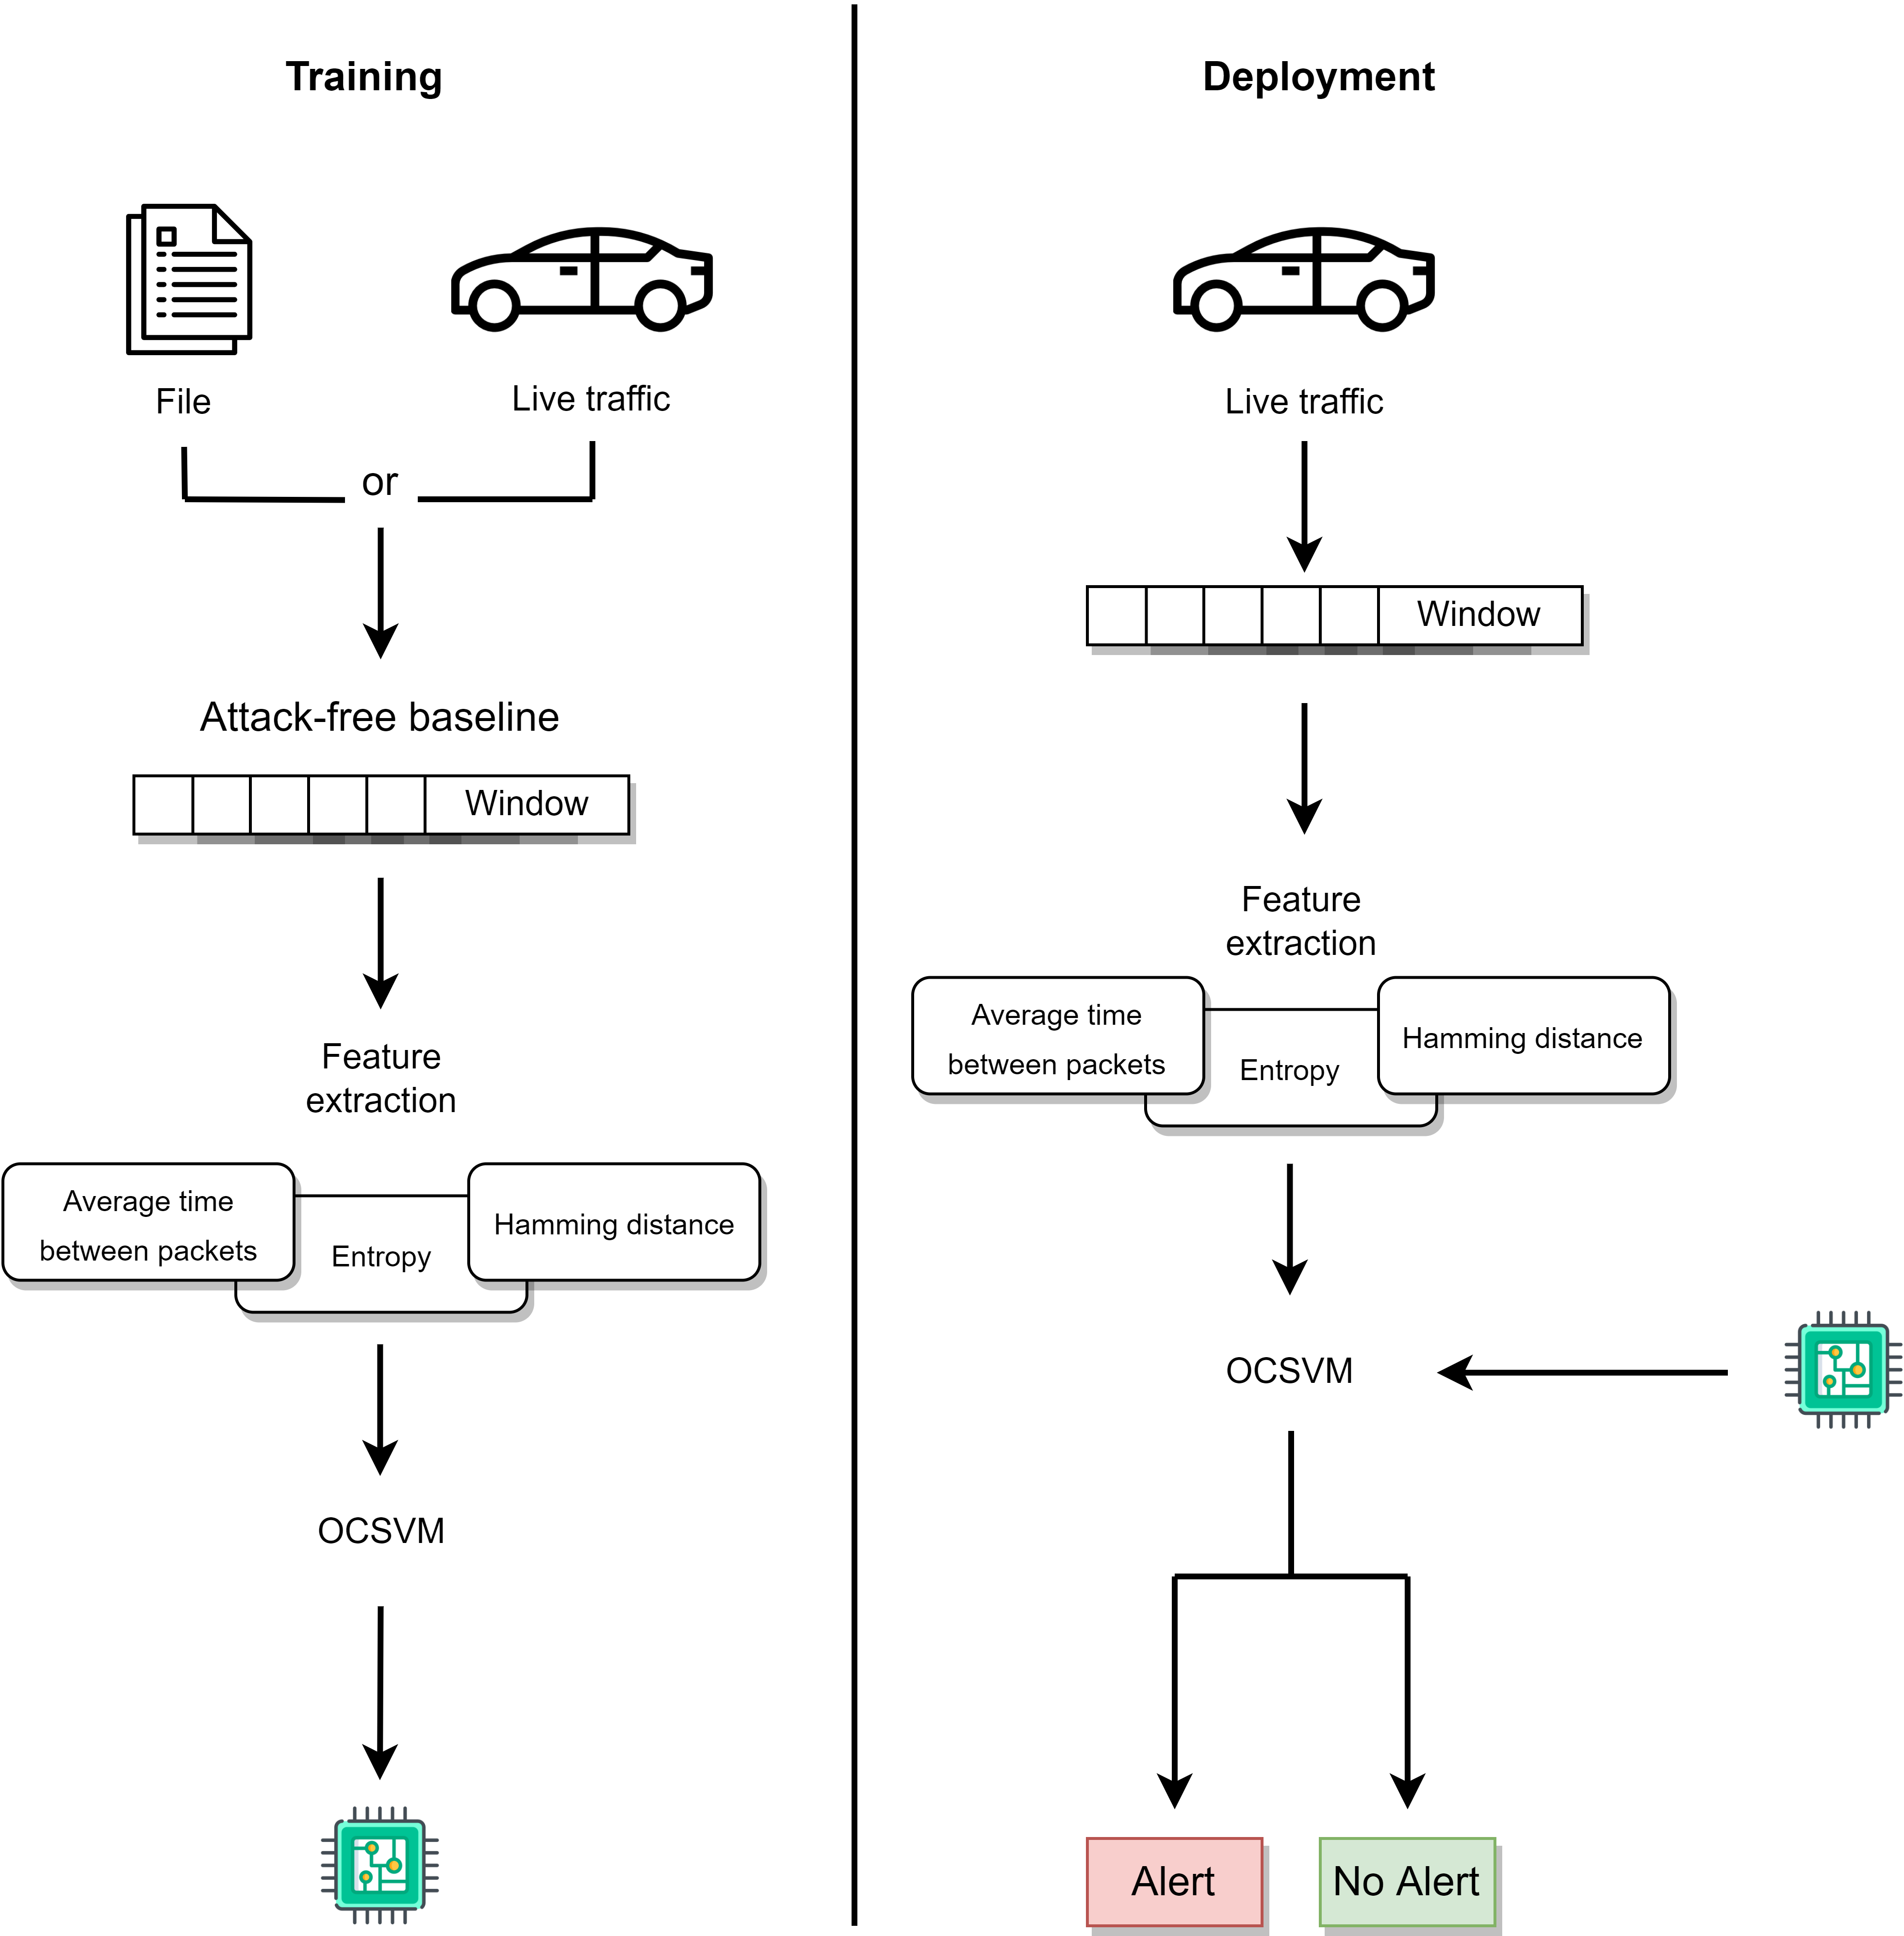
\includegraphics[width = \textwidth]{img/parts/app/IDS.png}
    \caption{IDS architecture}
    \label{fig:ids_architecture}
\end{figure}

\section{Training}
\label{sec:app_training}

Training the \gls{ids} can be done both in an online and offline fashion. Training online means that a baseline reading is gathered from live traffic, which must be attack-free to generate an accurate model because attacks are detected based upon significant deviations from the baseline traffic's characteristics. Offline training is done by providing the \gls{ids} with a \gls{csv} file containing CAN traffic that will serve as a baseline.\par
Features are extracted using a rolling window on the collected traffic, which are then scaled to fit in the [0, 1] interval. The minimum and maximum values of each feature are saved to perform proper feature scaling when the \gls{ids} is deployed.\par
The kernel method is employed using the Gaussian kernel with $\epsilon = 1$ and the model is trained with the $\nu$ parameter set to 0.01. The \gls{ids} is then saved to the filesystem so it can be recovered upon a system restart. The documentation for the structure and training function can be seen in Figures \ref{fig:ids_struct} and \ref{fig:ids_train}, respectively.

\begin{figure}
    \centering
    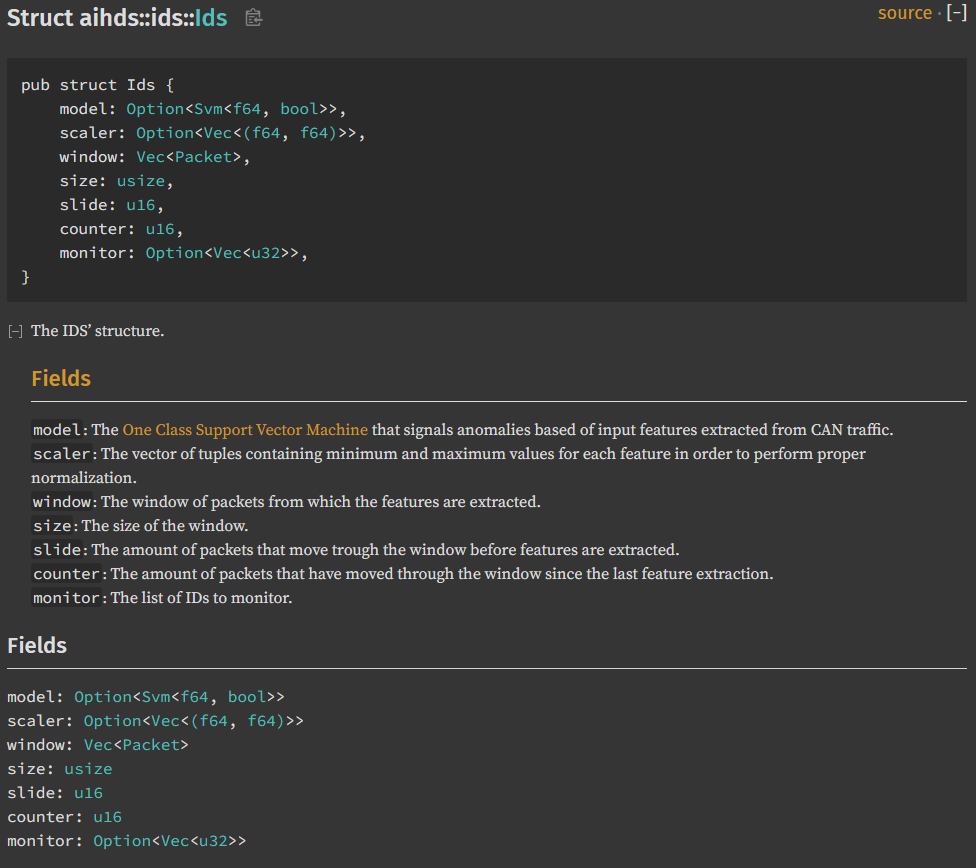
\includegraphics[width = \linewidth]{img/parts/docs/ids/ids_struct.png}
    \caption{\gls{ids} structure}
    \label{fig:ids_struct}
\end{figure}

\begin{figure}
    \centering
    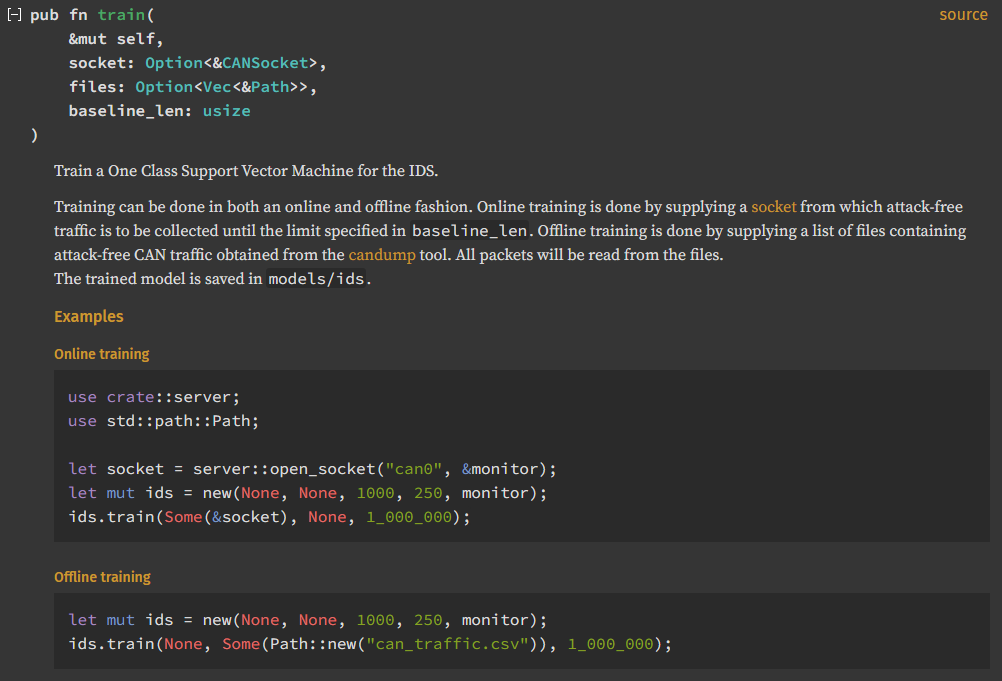
\includegraphics[width = \linewidth]{img/parts/docs/ids/ids_struct_train.png}
    \caption{Training function}
    \label{fig:ids_train}
\end{figure}

% \begin{itemize}
%     \item \textit{model}: The \gls{ocsvm}
%     \item \textit{scaler}: A vector of tuples containing the minimum and maximum values of each feature from the baseline
%     \item \textit{window}: The collection of packets from which features are extracted
%     \item \textit{size}: The amount of packets the window can hold
%     \item \textit{slide}: The amount of packets that leave and enter the window in a FIFO fashion
%     \item \textit{counter}: The number of packets that have left and entered the window between slides
%     \item \textit{monitor}: The collection of IDs to monitor
% \end{itemize}

\section{Features}
\label{sec:app_features}

This section focuses on the features extracted from \gls{can} bus traffic that are then used as input to the \gls{ocsvm} model. Prior research on \glspl{ids} that focus on \gls{can} has found success in the use of frequency analysis and information-theoretic algorithms, as shown in Section \ref{sec:can_ids}. Frequency analysis was one of the first methods used to detect packet insertion attacks. Since many packets of the same ID are sent at a consistent interval (typically 10 or 20 milliseconds), a variation of these timings caused by a bad actor inserting packets into the network would be picked up as an anomaly. On the other hand, information-theory may aid in detecting anomalous behaviour caused by packet modification attacks, or packet low-frequency packet insertion.\par
Here, the proposed features are described, and the feature selection process is presented.

\subsection{Packet frequency}

Frequency analysis consists of measuring the average time between consecutive packets with the same ID. Since many packets sharing the same ID are sent at regular intervals, an attacker inserting new packets into the network would decrease the time between packets, which would be detected by the \gls{ids}. Likewise, packet suppression would also trigger an alert.\par
Calculating the arrival time between packets can done by \[T(p_{t_0}, p_{t_1}) = t_1 - t_0\] where $t_0$ and $t_1$ are consecutive arrival timestamps for packets of the same ID.

\subsection{Shannon entropy}

In the \gls{can} domain, traffic is more restricted than in standard computer networks. This means that, generally, entropy in an automotive network is lower \citep{muter2011entropy}. If an attacker replaces the payload of a given ID, it likely would change the network entropy, triggering an alert (an instance of this would be a constant payload on an ID that usually sends distinct values, or vice-versa).\par
The concept of information entropy was first introduced by \cite{shannon1948}. Shannon entropy is often defined as being the amount of information or uncertainty of a random variable. For an alphabet $X$, and a random variable $x \in X$ distributed according to $p: x \rightarrow [0, 1]$, Shannon entropy is defined as \[H(X) = - \sum_{i - 1}^{n} P(x_i) \log_2 P(x_i)\]\par
An occurrence with probability 1 has no entropy, while a set of occurrences with a balanced probability distribution has an entropy value of 1. 

\subsection{Hamming distance}

In information theory, the number of points where the matching symbols are different between two strings of equal length is known as the Hamming distance \citep{hamming1950}. For example, the Hamming distance between 0000 and 1111 is 4, while the Hamming distance between 0101 and 1101 is 1. The formula for evaluating the Hamming distance between two words of length $k$ is \[H_d(x, y) = \sum_{i = 1}^{k} \vert x_i - y_i \vert\]\par

Here, the proposed approach consists on calculating the Hamming distance between consecutive packets in the network, similar to what was proposed by \cite{stabili2017}. The authors formulated this as being \[H_d(p_t, p_{t + 1}) = \sum_{i = 1}^{k} p_{t}^{i} \otimes p_{t + 1}^{i}\] where $p_t$ is a generic payload at time $t$ and $p_t^i$ is the $i_{th}$ element of that payload.

Both bit and byte-wise calculations were explored in the development of this prototype. An example of a bit-wise Hamming distance calculation is \[H_{bit}(0000000\ 000110100, 00111111\ 00000100) = 8\]
and the same operation performed byte-wise is \[H_{byte}(00\ 34, 3F\ 04) = 2\]

\subsection{Difference between bytes}

The calculation of the difference between bytes is done by \[D(p_t, p_{t+1}) = \sum_{i = 1}^{k} \vert p_t^i - p_t^{i+1} \vert \] where $p_t$ is a generic payload at time $t$ and $p_t^i$ is the $i_{th}$ element of that payload.\par
The hypotheses is that this metric, similar to entropy and Hamming distance, contributes to the modelling of what constitutes normal packet payload behaviour.

\subsection{Selection}

For all datasets, five features were extracted from each rolling window of traffic: average frequency, average entropy, average bit-wise Hamming distance, average byte-wise Hamming distance, and average byte-wise difference. Since it would take a lot of computational power to extract all five features from each window while keeping up with incoming traffic, dimensionality reduction was performed. To do so, correlation between features and the datasets' labels was calculated. Some illustrative results are shown in Figure \ref{fig:fe}, with all results obtained being present in Appendix \ref{apdx:sec:feature_selection}. All features were extracted from a 1000 packet rolling window, with a slide of 250 packets.\par

Figure \ref{fig:fe} shows some illustrative examples of how these features are correlated with each other and the label. In the case of a modification attack, payload behavior will be altered, but no packets will be inserted. This is demonstrated in Figure \ref{subfig:fe_crysys_incr}, where the average time between packets (\emph{AvgTime}) shows no correlation with the dataset's label, but both entropy and Hamming distance-related features show a higher correlation. Figure \ref{subfig:fe_ieee_challende_d} shows feature correlation values in the case where a variety of spoofing, replay, fuzzing, and flooding attacks are performed. All features except the difference between consecutive payloads of the same ID (\emph{GapBytes}) show some correlation with the label, meaning that they are relevant predictors of many common attacks. Lastly, Figure \ref{subfig:fe_tue_opelastra} shows feature correlation values in the case of a replay attack. Here, only the average time between packets is relevant, since many previously observed packets are being inserted into the \gls*{can} bus. Payload-related features show no correlation with the label, which is to be expected because the attack consists of inserting packets whose payload is not abnormal.

\begin{figure}
    \centering
    
    \begin{subfigure}[b]{.6\linewidth}
        \centering
        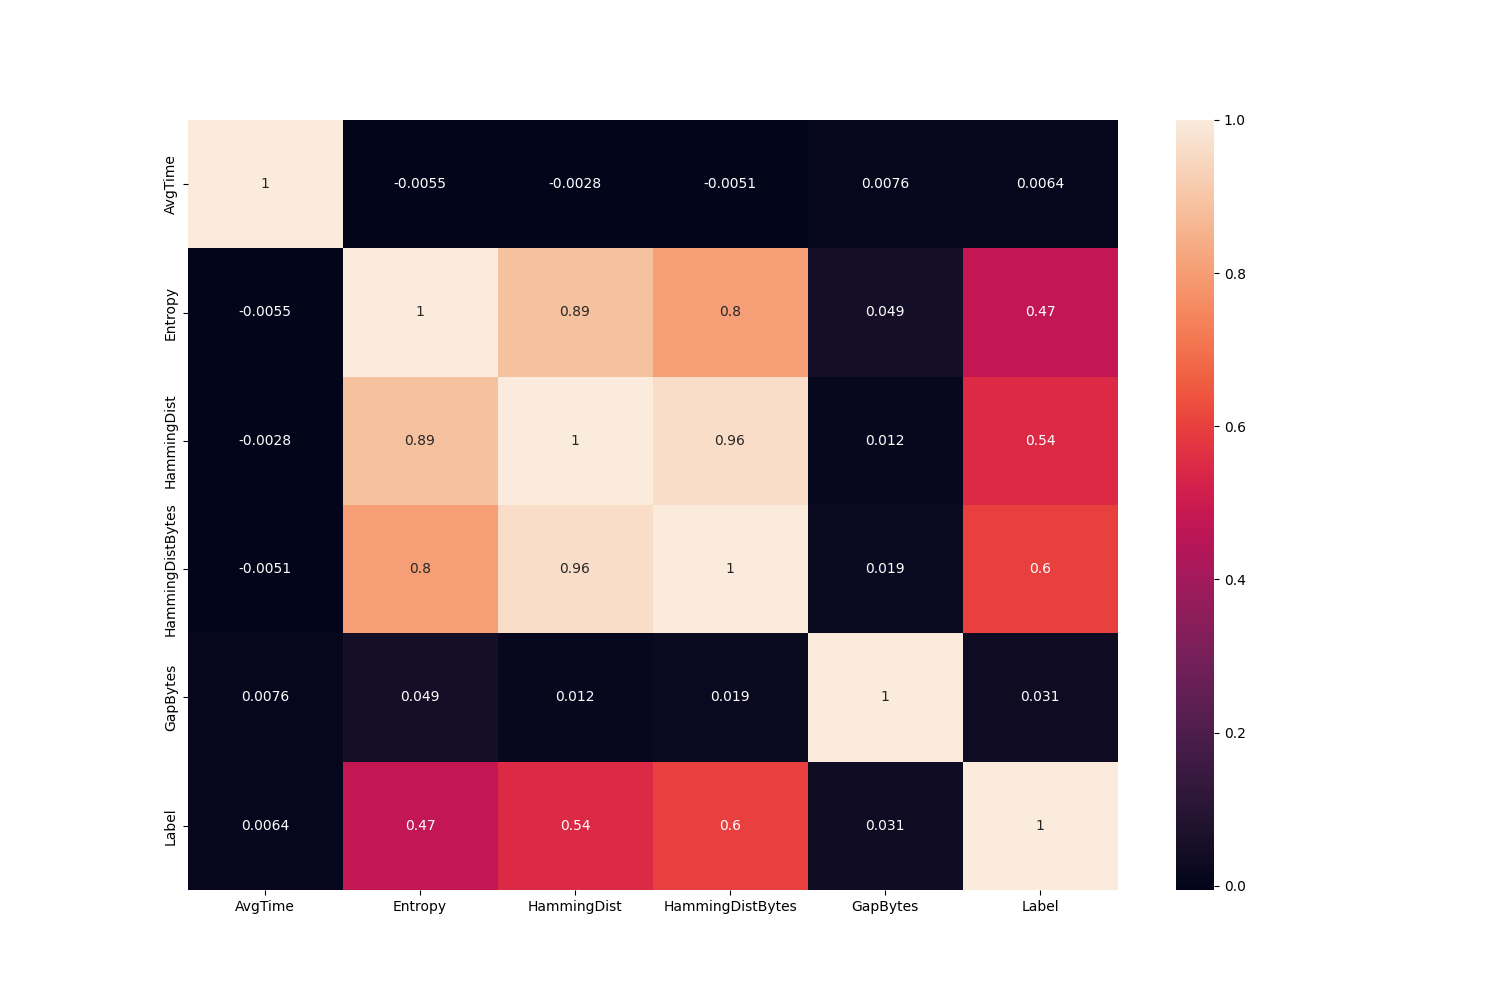
\includegraphics[width = \linewidth]{img/parts/app/feature_correlation/crysys/incr.png}
        \caption{CrySyS Lab - Adding an incrementing amount to packet payload}
        \label{subfig:fe_crysys_incr}
    \end{subfigure}
    
    \begin{subfigure}[b]{.6\linewidth}
        \centering
        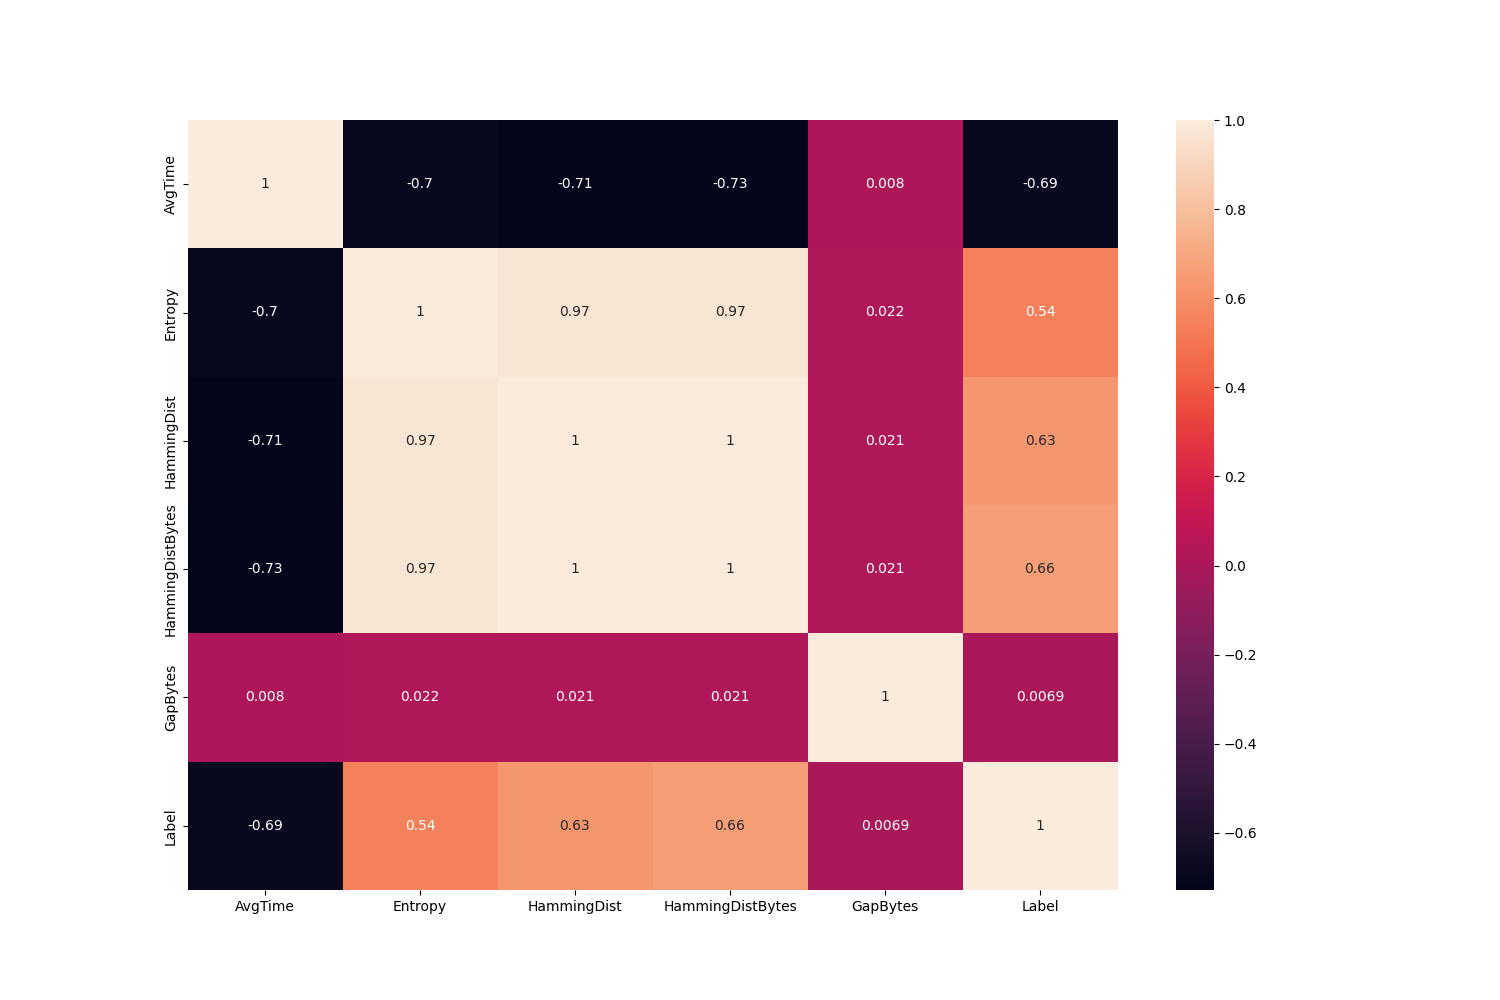
\includegraphics[width = \linewidth]{img/parts/app/feature_correlation/ieee_challenge/pre_submit_D.png}
        \caption{IEEE Car Hacking: Attack \& Defense Challenge 2020 - Attacks while driving}
        \label{subfig:fe_ieee_challende_d}
    \end{subfigure}
    
    \begin{subfigure}[b]{.6\linewidth}
        \centering
        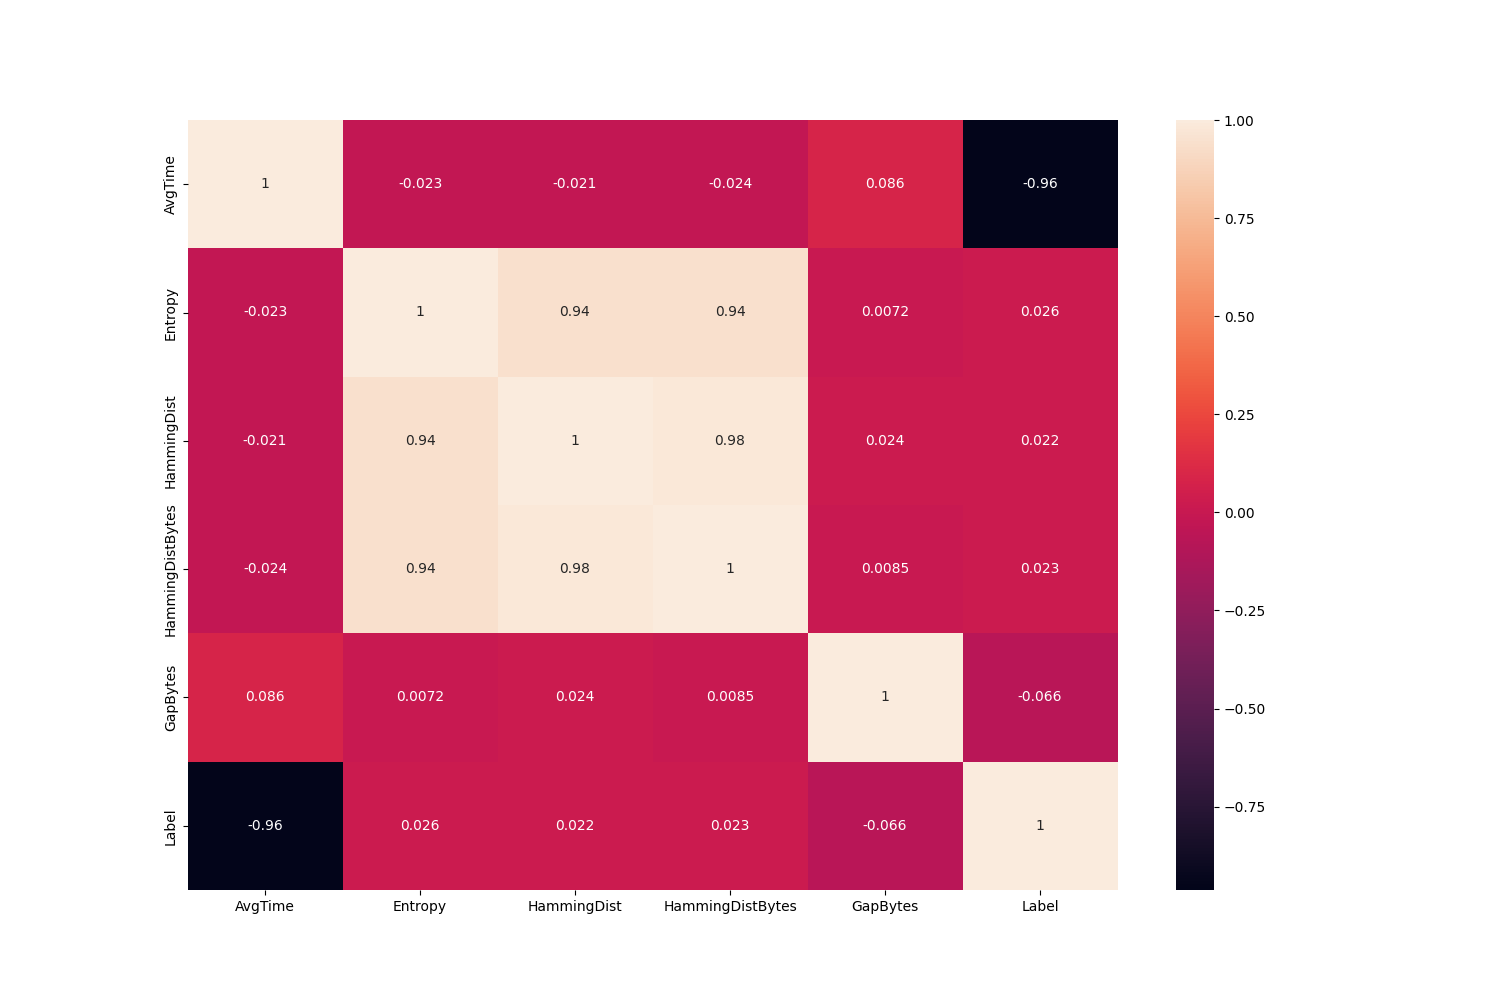
\includegraphics[width = \linewidth]{img/parts/app/feature_correlation/OpelAstra/replay.png}
        \caption{Automotive Controller Area Network (CAN) Bus Intrusion Dataset v2 - Replay attack}
        \label{subfig:fe_tue_opelastra}
    \end{subfigure}
    
    \caption{Correlation between extracted features}
    \label{fig:fe}
\end{figure}

Thus, after observing several attack types, including with and without packet insertion, the average byte-wise Hamming distance and the average arrival time between packets of the same ID appear to be the most promising in predicting whether an attack is present or not.

\section{Embedded system environment}
\label{sec:app_embedded}

To simulate the environment where the proposed system would be deployed, the program was written in Rust 1.62.0 and compiled to the ARM v7 architecture to run on a Raspberry Pi 4 Model B connected to the ECU cluster shown in Figure \ref{fig:setup}. Code documentation is available in Appendix \ref{apdx:sec:code_documentation}, with additional Python tools that assisted in development being detailed in Appendix \ref{apdx:sec:tools}.\par

To verify if the system would be able to analyse real-time traffic, the number of packets per second it was able to process was recorded. This came at around 1600. However, it was unclear whether this was a bottleneck or if it was the real network throughput. To clear this, traffic was logged onto a \gls{csv} file and processed by the Raspberry Pi as if it was live traffic, but read from memory instead of a network socket. The average number of packets per second processed came at 39,195.426, while the average number of packets per second in the log file was 1,678.878. The proposed system should therefore be able to perform real-time analysis in an embedded environment. CPU usage was recorded as being 5\%, signalling that its implementation in a real ECU would not raise serious concerns about resource usage.\par
It is also important to assure that the algorithm does not consume too much power, as it would reduce the overall range of the vehicle. Figure \ref{fig:powerdraw} shows how much current the Raspberry Pi was drawing while executing the \gls{ids}. Applied voltage was constant at 4900mV. The baseline current was established to be at 400mA, and it rose up to 500mA when the \gls{ids} was executing. This comes at 0.5W, which is negligible.

\begin{figure}
    \centering
    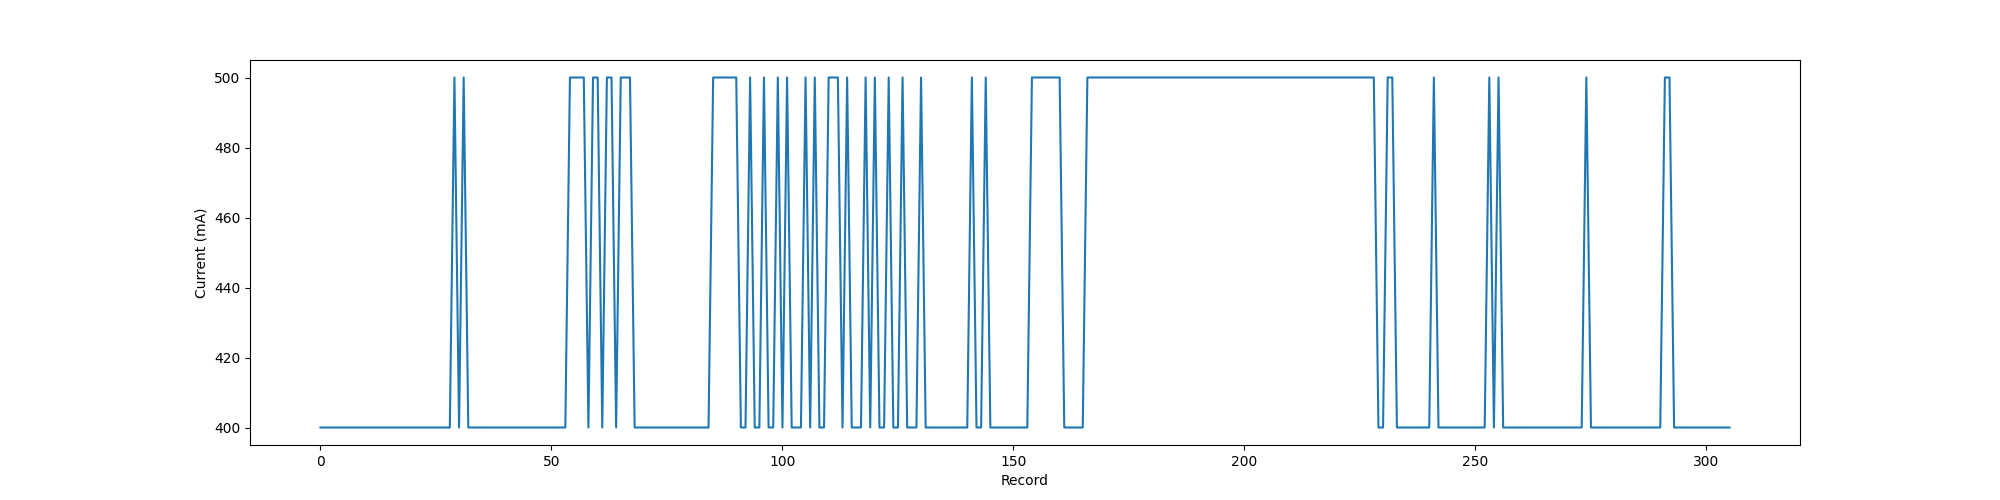
\includegraphics[width = \linewidth]{img/parts/app/powerdraw.png}
    \caption{Power consumption from the Raspberry Pi while executing the proposed \gls{ids}}
    \label{fig:powerdraw}
\end{figure}

\section{Execution}
\label{sec:app_exe}

A \gls{cli} was developed in order to facilitate application testing and deplyment. It consists of the following:

\begin{verbatim}
USAGE:
    aihds [OPTIONS]

OPTIONS:
        --extract-features <EXTRACT_FEATURES>
            Extracts features to CSV files
    -h, --help
            Print help information
        --live
            Run IDS in live mode
        --model <MODEL>
            Path to model to be loaded
        --monitor <LIST>
            IDs to monitor
        --streaming <URL>
            Run model in streaming mode
        --test <PATHS>
            Paths to the datasets required for testing the model,
            separated by ','
        --train <PATHS>
            Paths to the datasets required for training the model,
            separated by ','
    -V, --version
            Print version information
\end{verbatim}

Running the application in online mode is done with the \emph{live} option, while the \emph{training} option is used to indicate the file on which offline training will be performed. The \emph{streaming} option sends features and predictions as HTTP requests to the specified \gls{url}. An example of a graphical interface to visually represent the streaming data can be seen on Figure \ref{fig:website}.

\begin{figure}
    \centering
    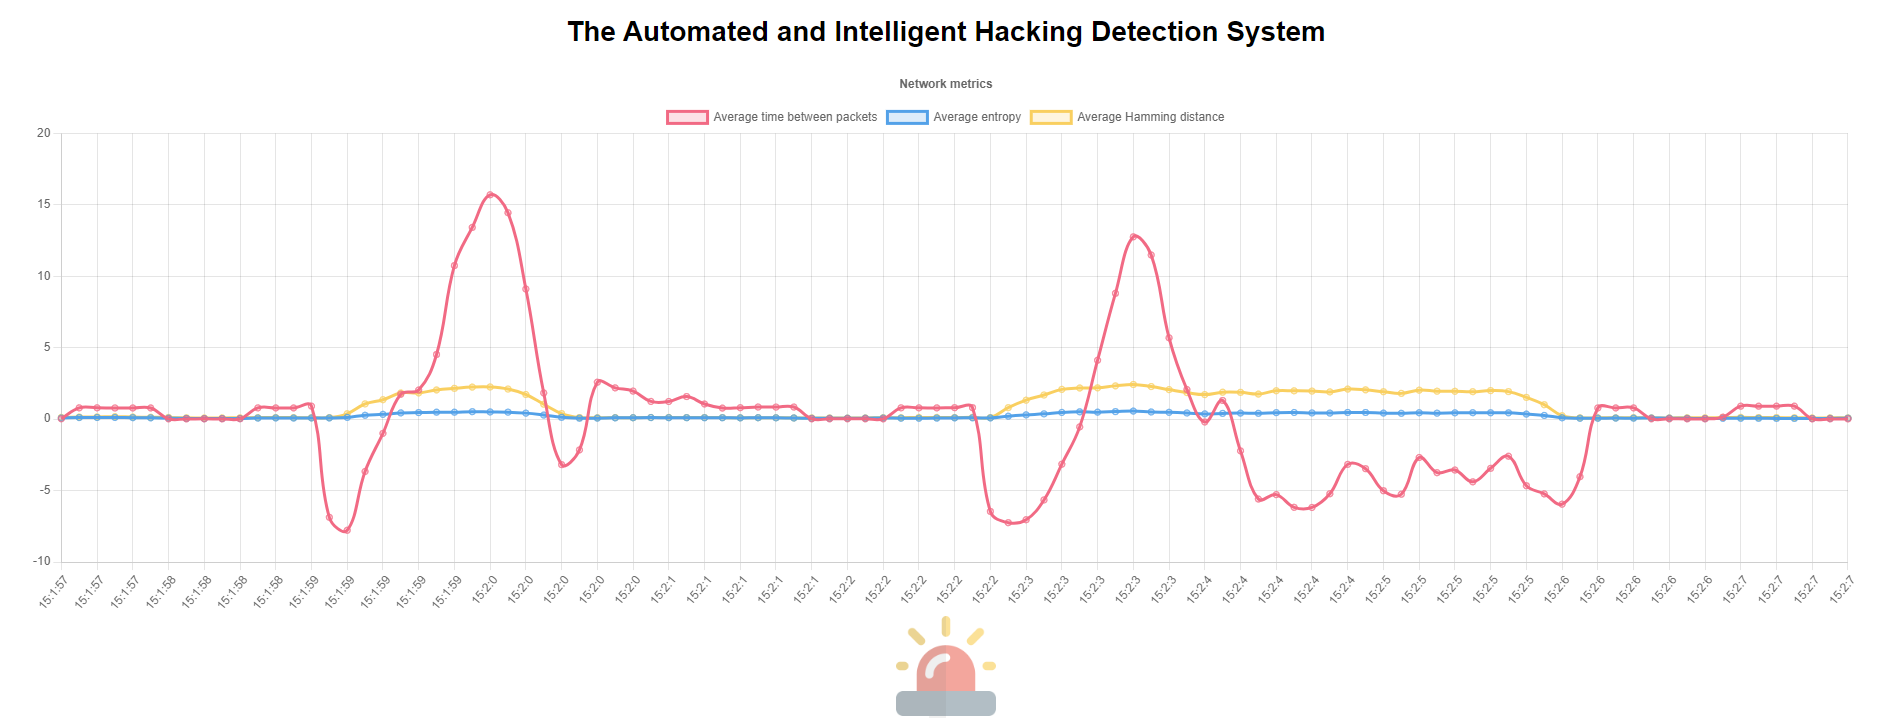
\includegraphics[width = \linewidth]{img/parts/app/website.png}
    \caption{Graphical interface}
    \label{fig:website}
\end{figure}